% =============================================================================
% MAL Omics: Tables, Figures, and Key Results
% COPDGene Plasma Proteomics
% =============================================================================
\documentclass[11pt, letterpaper]{article}

\usepackage[margin=1in]{geometry}
\usepackage{amsmath}
\usepackage{booktabs}
\usepackage{array}
\usepackage{caption}
\usepackage{float}
\usepackage{graphicx}
\usepackage{hyperref}
\usepackage{xcolor}
\usepackage{multirow}
\usepackage{parskip}
\usepackage{subcaption}
\graphicspath{{../figures/}}

\setlength{\parskip}{6pt}

\newcommand{\missing}[1]{\textcolor{red}{\textit{Not found: #1}}}

% =============================================================================
\begin{document}

\begin{center}
  {\Large \textbf{MAL Omics: Proteomics Analysis Report}} \\[4pt]
  {\normalsize COPDGene, SomaScan ($\sim$4,979 proteins), $n = 1{,}306$}
\end{center}

\vspace{6pt}
\noindent\textbf{Study.}
COPDGene is a longitudinal cohort study of current and former smokers
enrolled at 21 US clinical centers. Subjects were seen at Phase~2
($\sim$2013--2017) and Phase~3 ($\sim$2019--2022), approximately
5--6 years apart. Blood was drawn at Phase~2 and
profiled by SomaScan, an aptamer-based platform that quantifies
$\sim$4,979 plasma proteins simultaneously as RFU (Relative Fluorescence
Units). This analysis uses $n = 1{,}306$ subjects with complete
proteomics, phenotype, and MAL data.

\noindent\textbf{MAL (Mechanically Affected Lung).}
Computed tomography (CT)-derived continuous score (range 0.01--0.40)
measuring the fraction of lung volume under destructive mechanical
stress. Higher MAL = more lung tissue under stress. MAL is computed from
inspiratory/expiratory CT image registration and is distinct from
standard emphysema measures (e.g., \%LAA-950). Variable name in data:
\texttt{meanmal}.

MAL is itself a strong predictor of who will develop worse emphysema
over time: higher mechanical stress on lung tissue drives progressive
structural damage. However, MAL requires specialized CT analysis and is
not available from a routine blood draw.

\noindent\textbf{Goal.}
(1) Identify which Phase~2 plasma proteins are associated with MAL,
establishing that mechanical lung stress leaves a detectable signal
in blood.
(2) Use those proteins to build a Proteomic Risk Score (proRS) from a
Phase~2 blood draw that approximates MAL and can predict who will
develop worse emphysema by Phase~3. If successful, the proRS would
allow MAL-like risk stratification without requiring CT image
registration. The proteins themselves are not measured at Phase~3;
they serve as baseline predictors of the CT density change that
occurs between visits ($\sim$6 years apart).

\noindent\textbf{Outcome.}
Emphysema progression = change in CT lung density Phase~3 $-$ Phase~2
(\texttt{Change\_lung\_\allowbreak density\_\allowbreak vnb\_\allowbreak P2\_\allowbreak P3},
Hounsfield Units [HU]). Negative = worsened. Mean $\approx 1$ HU
(standard deviation [SD] 7) in this cohort; a negative value means the
lung became less dense (more emphysematous) between visits.

% =============================================================================
\section*{Data Sources and Variable Names}

Four CSV files were used. All joins are on \texttt{sid}.

\subsection*{\texttt{data/csv\_exports/prot.csv}: SomaScan proteomics}

\begin{tabular}{p{3.5cm}p{10cm}}
\toprule
Column & Description \\
\midrule
\texttt{sid}             & Subject identifier (join key) \\
\texttt{X\{seqID\}}      & Raw RFU value for each protein (e.g.\ \texttt{X10000.28}).
                           $\sim$4,979 columns matching pattern \texttt{\^{}X[0-9]}.
                           Renamed to \texttt{log2\_X\{seqID\}} after log$_2$ transform. \\
\bottomrule
\end{tabular}

\subsection*{\texttt{data/csv\_exports/pheno\_MAL.csv}: Phenotypes and covariates}

\begin{tabular}{lll}
\toprule
Column & Used as & Status \\
\midrule
\texttt{sid}                          & Join key            & Found \\
\texttt{Change\_lung\_density\_vnb\_P2\_P3} & Outcome: emphysema progression (HU) & Found \\
\texttt{lung\_density\_vnb\_P2}       & Baseline lung density (HU)  & Found \\
\texttt{Age\_P2}                      & Age (years)                 & Found \\
\texttt{gender}                       & Sex (coded 1/2)             & Found \\
\texttt{race}                         & Race (coded 1/2)            & Found \\
\texttt{ATS\_PackYears\_P2}           & Pack-years of smoking       & Found \\
\texttt{SmokCigNow\_P2}               & Current smoking (0/1)       & Found \\
\texttt{scanner\_model\_clean\_P2}    & CT scanner model            & Found \\
\texttt{FEV1\_FVC\_post\_P2}          & FEV$_1$ (forced expiratory volume in 1 second) / FVC (forced vital capacity) ratio & Found \\
\texttt{PC1} -- \texttt{PC5}          & Ancestry principal components & Found \\
\texttt{fev1\_pp\_gli\_global\_P2}      & FEV$_1$\% predicted (GLI global reference) & Found \\
\texttt{BMI\_P2}                      & Body mass index             & See \texttt{CellData.csv} below \\
\bottomrule
\end{tabular}

\subsection*{\texttt{data/Data/MAL.csv}: MAL scores}

\begin{tabular}{ll}
\toprule
Column & Description \\
\midrule
\texttt{sid}      & Subject identifier (join key) \\
\texttt{meanmal}  & MAL score (continuous, range 0.01--0.40) \\
\bottomrule
\end{tabular}

\subsection*{\texttt{data/csv\_exports/CellData.csv}: Phase 2 BMI}

\begin{tabular}{lll}
\toprule
Column & Used as & Note \\
\midrule
\texttt{sid}          & Join key   & \\
\texttt{Phase\_study} & Phase filter & Rows with \texttt{Phase\_study == 2} used \\
\texttt{BMI}          & \texttt{BMI\_P2} in analysis & All 1,306 analysis subjects present, no missingness \\
\bottomrule
\end{tabular}

\subsection*{\texttt{data/csv\_exports/metadat5k.csv}: Protein annotation}

\begin{tabular}{ll}
\toprule
Column & Description \\
\midrule
\texttt{seqID}              & Protein sequence identifier; joins to \texttt{log2\_X\{seqID\}} \\
\texttt{EntrezGeneSymbol}   & HGNC (HUGO Gene Nomenclature Committee) gene symbol (e.g.\ \texttt{ADIPOQ}) \\
\texttt{Target}             & Short protein name (e.g.\ \texttt{Adiponectin}) \\
\texttt{TargetFullName}     & Full protein name \\
\bottomrule
\end{tabular}

\vspace{8pt}
\noindent\textbf{Join logic.} Three-way inner join:
\texttt{prot} $\bowtie_{\texttt{sid}}$ \texttt{pheno} $\bowtie_{\texttt{sid}}$ \texttt{MAL}.
Metadata joined on \texttt{seqID = sub("\^{}log2\_X", "", predictor)}.

File sizes: \texttt{prot.csv} has 5,670 subjects; \texttt{MAL.csv}
has 5,024 subjects; \texttt{pheno\_MAL.csv} has 10,652 subjects.
After the 3-way inner join on \texttt{sid}: $n = 4{,}630$.

Complete-case filter then requires non-missing values for all of:
\texttt{Change\_lung\_density\_vnb\_P2\_P3} (Phase~3 outcome),
\texttt{lung\_density\_vnb\_P2}, \texttt{meanmal}, \texttt{Age\_P2},
\texttt{gender}, \texttt{race}, \texttt{ATS\_PackYears\_P2},
\texttt{SmokCigNow\_P2}, \texttt{scanner\_model\_clean\_P2},
\texttt{fev1\_pp\_gli\_global\_P2},
\texttt{FEV1\_FVC\_post\_P2}, and \texttt{PC1}--\texttt{PC5}.

This reduces the sample to $n = 1{,}306$. The large drop
($4{,}630 \to 1{,}306$) is driven primarily by the Phase~3 outcome:
8,912 of 10,652 subjects in \texttt{pheno\_MAL.csv} (84\%) have no
Phase~3 CT scan recorded, meaning they did not return for the
follow-up visit $\sim$6 years later.

\bigskip
% =============================================================================
\section*{Table 1: Demographics}

\noindent Study population after 3-way merge (proteomics $\times$
phenotype $\times$ MAL) and complete-case filtering.

\begin{table}[H]
\centering
\caption*{\textbf{Table 1.} Baseline characteristics of COPDGene
  participants included in the proteomics analysis ($n = 1{,}306$).
  Subjects had complete SomaScan plasma proteomics, phenotype data, and
  MAL score. Continuous variables: mean (SD); categorical: $n$ (\%).
  MAL (Mechanically Affected Lung) = CT-derived score (range
  0.01--0.40); higher values indicate more lung under destructive
  mechanical stress. Emphysema progression = CT lung density at
  Phase~3 minus Phase~2 ($\rho_{\text{P3}} - \rho_{\text{P2}}$, HU);
  negative values indicate worsening.}
\begin{tabular}{lc}
\toprule
Characteristic & Overall ($n = 1{,}306$) \\
\midrule
\textit{Demographics} & \\
\quad Age (years)                         & 65 (8) \\
\quad Sex: male / female                  & 633 (48\%) / 673 (52\%) \\
\quad Race: White / Black                 & 991 (76\%) / 315 (24\%) \\
\addlinespace
\textit{Smoking} & \\
\quad Current smoker                      & 445 (34\%) \\
\quad Pack-years                          & 43 (23) \\
\addlinespace
\textit{Pulmonary function} & \\
\quad FEV\textsubscript{1}\% predicted (GLI global) & 83 (24) \\
\quad FEV\textsubscript{1}/FVC            & 0.69 (0.14) \\
\addlinespace
\textit{CT imaging} & \\
\quad Lung density Phase 2 (HU)           & 83 (23) \\
\quad MAL score                           & 0.04 (0.05) \\
\quad Emphysema progression (HU)          & 1 (7) \\
\addlinespace
\textit{Anthropometrics} & \\
\quad BMI (kg/m\textsuperscript{2})       & 29 (6) \\
\bottomrule
\end{tabular}
\end{table}

\noindent\textit{Note.} Sex is coded 1/2 in the data; assumed Male/Female
per COPDGene convention. Race coded 1/2; assumed White/Black. Emphysema
progression mean of 1 HU (SD 7) reflects a near-zero mean; the
distribution includes both progressors (negative $\Delta\rho$) and
improvers (positive $\Delta\rho$).

% =============================================================================
\section*{Figure 1: Study Design}

\noindent Requires a schematic (e.g., BioRender) illustrating the analysis flow:
SomaScan proteomics $\to$ differential expression $\to$ GSEA (Gene Set
Enrichment Analysis) / STRING $\to$ adaptive LASSO (Least Absolute
Shrinkage and Selection Operator) proRS (Proteomic Risk Score) $\to$
emphysema progression association $\to$ causal mediation.

\begin{figure}[H]
  \centering
  \fbox{\parbox{0.85\textwidth}{\centering\vspace{2cm}
    \textit{[Figure 1 placeholder: study design schematic to be
    drawn manually, e.g., BioRender]}
  \vspace{2cm}}}
  \caption{Overview of the COPDGene MAL omics analysis pipeline.
    SomaScan plasma proteomics ($\sim$4,979 proteins, Phase~2) are used
    to identify proteins associated with MAL (differential expression,
    GSEA, STRING network), build a proteomic risk score (adaptive LASSO),
    test whether the score predicts emphysema progression (Phase~3
    minus Phase~2 CT density), and quantify mediation of the MAL effect
    through blood proteins (causal mediation analysis).}
\end{figure}

% =============================================================================
\section*{Figure 2: Protein Expression Landscape of MAL}

\subsection*{A. Volcano Plot (protein $\sim$ MAL)}

Each dot is one protein. The $x$-axis ($\hat\beta$) shows how much a
protein changes per one-unit increase in MAL after adjusting for age,
sex, race, smoking, pack-years, BMI, scanner, and ancestry PCs. Positive
$\hat\beta$ = protein is higher with more mechanical lung stress;
negative = lower. $\hat\beta$ is defined as the change in log$_2$
protein per \emph{one-unit} increase in MAL. But MAL only ranges from
0.01 to 0.40 in this cohort, so a one-unit change never actually
occurs. To express the effect in realistic terms, multiplying
$\hat\beta$ by the full MAL range ($0.40 - 0.01 = 0.39$) gives the
maximum expected protein change across the entire observed spread of
MAL. For TNNT2 (Troponin~T, the most significant protein):
$0.227 \times 0.39 \approx 0.09$ log$_2$-unit shift from the lowest
to the highest MAL subject. The $y$-axis ($-\log_{10}$ $p$-value) is
confidence: higher = more significant. The dashed horizontal line
marks the FDR $< 0.05$ threshold on the $p$-value scale. Dots above
the threshold are coloured red (enriched) or blue (depleted); grey
dots did not reach significance.
A dot far right and high = reliably elevated with more MAL.
A dot far left and high = reliably lower with more MAL.

\textbf{How calculated.}
For each of 4,979 proteins:
\[
  \log_2(\text{protein}) \;\sim\;
  \beta_{\text{MAL}} \cdot \texttt{meanmal}
  \;+\; \text{age} + \text{sex} + \text{race}
  + \text{pack-years} + \text{smoking}
  + \text{BMI} + \text{scanner} + \text{PC1--PC5}
\]
$\hat\beta_{\text{MAL}}$ = change in log$_2$ protein level per one-unit
increase in MAL. FDR correction (Benjamini--Hochberg) across all 4,979
tests. FEV$_1$\% predicted is intentionally excluded: airflow obstruction
lies on the causal pathway from mechanical stress to lung damage, so
adjusting for it would remove the signal of interest.

\textbf{Key result.} 14 of 4,979 proteins significant at FDR $<$ 0.05 (6 positively associated, 8 negatively associated).

\begin{figure}[H]
  \centering
  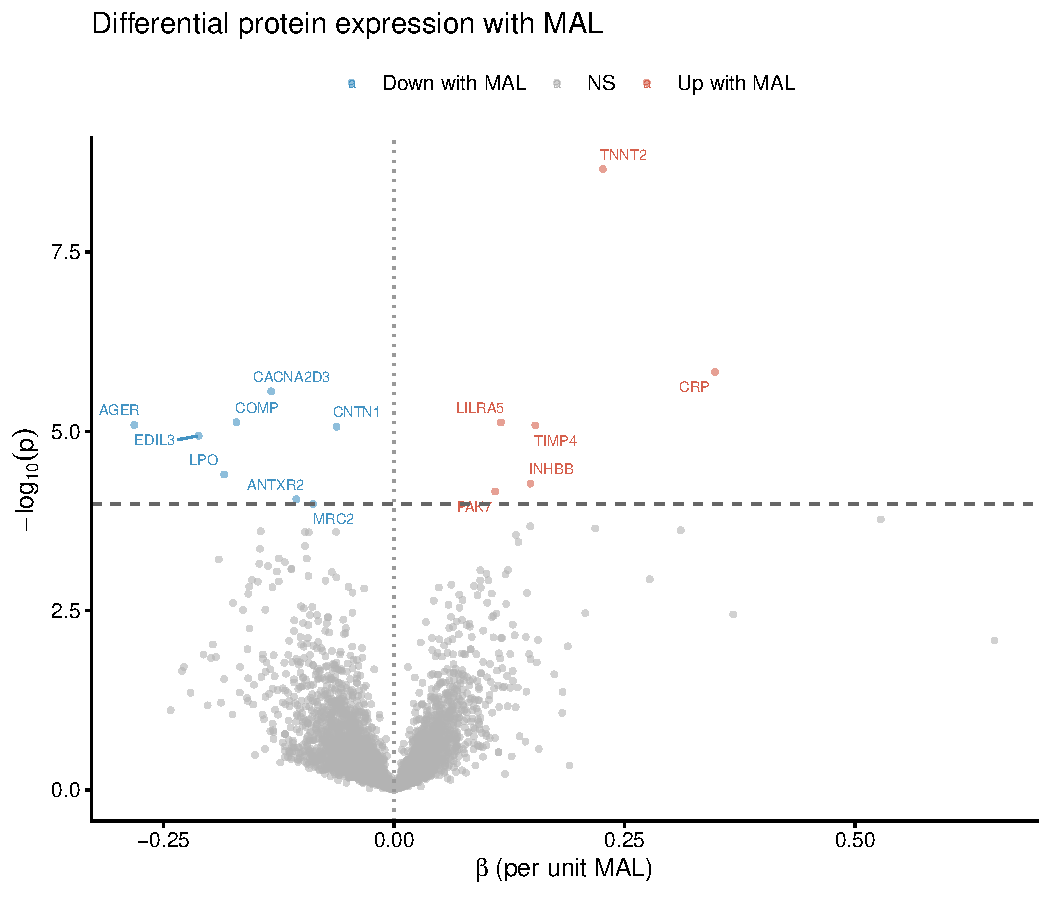
\includegraphics[width=0.85\textwidth]{Figure2A_volcano.pdf}
  \caption{Differential plasma protein expression associated with
    Mechanically Affected Lung (MAL) score in COPDGene participants
    ($n = 1{,}306$; 4,979 SomaScan proteins). Each point is one
    protein. $x$-axis: regression coefficient ($\hat\beta$) for
    log$_2$ protein level per unit MAL, adjusted for age, sex, race,
    pack-years, smoking, BMI, CT scanner, and ancestry PCs (PC1--PC5).
    $y$-axis: $-\log_{10}$($p$-value); dashed line = FDR $< 0.05$ threshold. Red = FDR
    $< 0.05$, positively associated; blue = FDR $< 0.05$, negatively
    associated; grey = not significant. Top 20 proteins by FDR
    labelled. 14 proteins reached FDR $< 0.05$ (6 positively, 8 negatively associated with MAL).}
\end{figure}

Top enriched (higher with more MAL, FDR $< 0.05$):
\textit{TNNT2} (Troponin~T, $\beta = 0.23$),
\textit{CRP} ($\beta = 0.35$),
\textit{TIMP4} ($\beta = 0.15$),
\textit{LILRA5} ($\beta = 0.12$),
\textit{INHBB} ($\beta = 0.15$),
\textit{PAK7} ($\beta = 0.11$).

Top depleted (lower with more MAL, FDR $< 0.05$, ordered by FDR):
\textit{CACNA2D3} ($\beta = -0.13$),
\textit{CNTN1} (contactin-1, $\beta = -0.06$),
\textit{AGER} (sRAGE, $\beta = -0.28$),
\textit{COMP} ($\beta = -0.17$),
\textit{EDIL3} ($\beta = -0.21$),
\textit{LPO} ($\beta = -0.18$),
\textit{ANTXR2} ($\beta = -0.11$),
\textit{MRC2} ($\beta = -0.09$).

% =============================================================================
\subsection*{A2. Sensitivity Analysis: Adjusting for CAD and CHF}

Several MAL-associated proteins (e.g., TNNT2, CRP) are established
cardiovascular biomarkers, raising the question of whether the observed
signals reflect cardiovascular comorbidity rather than mechanical lung
injury. To evaluate this, the primary differential expression analysis
was repeated with two additional covariates: history of coronary artery
disease (CAD; \texttt{CoronaryArtery\_P2}) and history of congestive
heart failure (CHF; \texttt{congestheartfail\_slv\_P2}), both ascertained at the Phase~2 visit from
\texttt{CellData.csv}. CAD and CHF data were complete for all
$n = 1{,}306$ analysis subjects (CAD: 7.5\%, $n = 98$;
CHF: 1.1\%, $n = 15$).

The model for each protein was:
\[
  \log_2(\text{protein}) \;\sim\; \text{MAL} + \text{age} + \text{sex}
  + \text{race} + \text{pack-years} + \text{smoking} + \text{BMI}
  + \text{scanner} + \text{PC1--PC5} + \text{CAD} + \text{CHF}
\]

Results are saved to \texttt{mal\_de\_sensitivity\_cad\_chf.csv}.

\textbf{Result.} All 14 proteins significant in the primary analysis
remained significant at FDR $< 0.05$ after CAD/CHF adjustment (100\%
overlap; 0 proteins lost). Regression coefficients were virtually
unchanged (median absolute $\Delta\hat\beta = 1.1\%$;
$r = 1.00$ between primary and adjusted estimates), indicating that
MAL-associated protein signals are not explained by prevalent
cardiovascular disease.

% =============================================================================
\subsection*{B. GSEA Barplot}

GSEA asks whether an entire biological pathway shows a coordinated shift
with MAL, rather than asking protein by protein. Each bar is one
significant pathway. Bar pointing right (NES $> 0$): the pathway's
proteins are on average higher in plasma with higher MAL. Bar pointing
left (NES $< 0$): lower. Longer bar = stronger shift. NES of $\pm 2$
is a strong, consistent signal. padj is the Benjamini--Hochberg
adjusted $p$-value across all pathways tested; only bars with padj $<
0.05$ are shown.

\textbf{How calculated.}
All 4,979 proteins ranked by their MAL $t$-statistic (most positively
associated at top, most negatively at bottom). Gene sets tested:
Hallmark, KEGG Legacy, Reactome (gene-set sizes 15--500).

NES (Normalized Enrichment Score): measures whether a gene set's
members concentrate at the top or bottom of the ranked list.
NES $> 0$ = enriched in high-MAL subjects; NES $< 0$ = depleted.
Normalization accounts for gene-set size so scores are comparable
across pathways.

padj (adjusted $p$-value): fgsea tests hundreds of pathways at once.
Without correction, many would appear significant by chance. padj is
the Benjamini--Hochberg correction applied within each gene set
collection (Hallmark, KEGG, Reactome separately). A padj $< 0.05$
means fewer than 5\% of pathways at this threshold are expected to be
false positives. Only pathways with padj $< 0.05$ are shown in the
barplot.

\textbf{Results.} 11 pathways significant (padj $< 0.05$). Eight are
depleted (NES $< 0$): glycosaminoglycan/keratan sulfate metabolism,
carbohydrate and lipid metabolism, biological oxidations,
branched-chain amino acid degradation, and fatty acid metabolism.
Three are enriched (NES $> 0$): antimicrobial peptides, chemokine
receptor signalling, and complement/coagulation cascades
(inflammatory/immune). Higher MAL is associated with lower
circulating metabolic proteins and higher inflammatory proteins.

\begin{table}[H]
\centering
\caption*{\textbf{Gene Set Enrichment Analysis (GSEA): significant
  pathways associated with MAL.} Proteins ranked by MAL $t$-statistic
  ($n = 4{,}979$) and tested using \texttt{fgsea} against Hallmark,
  KEGG Legacy, and Reactome gene sets (sizes 15--500). NES = Normalized
  Enrichment Score; NES $> 0$ = pathway proteins higher in high-MAL
  subjects (enriched); NES $< 0$ = lower (depleted). padj =
  Benjamini--Hochberg adjusted $p$-value within each collection.
  Only pathways with padj $< 0.05$ shown ($n = 11$).}
\begin{tabular}{llrr}
\toprule
Collection & Pathway & NES & padj \\
\midrule
Reactome & Diseases Assoc.\ with Glycosaminoglycan Metabolism & $-2.07$ & 0.011 \\
Reactome & Keratan Sulfate / Keratin Metabolism               & $-2.02$ & 0.022 \\
KEGG     & Valine, Leucine and Isoleucine Degradation         & $-2.03$ & 0.028 \\
Reactome & Biological Oxidations                              & $-1.85$ & 0.022 \\
Reactome & Sensory Perception                                 & $-1.86$ & 0.022 \\
Reactome & Diseases of Metabolism                             & $-1.87$ & 0.011 \\
Reactome & Metabolism of Carbohydrates and Derivatives        & $-1.76$ & 0.019 \\
Hallmark & Fatty Acid Metabolism                              & $-1.69$ & 0.039 \\
Reactome & Antimicrobial Peptides                             & $+2.06$ & 0.011 \\
Reactome & Chemokine Receptors Bind Chemokines                & $+2.19$ & 0.011 \\
KEGG     & Complement and Coagulation Cascades                & $+1.89$ & 0.028 \\
\bottomrule
\end{tabular}
\end{table}

\begin{figure}[H]
  \centering
  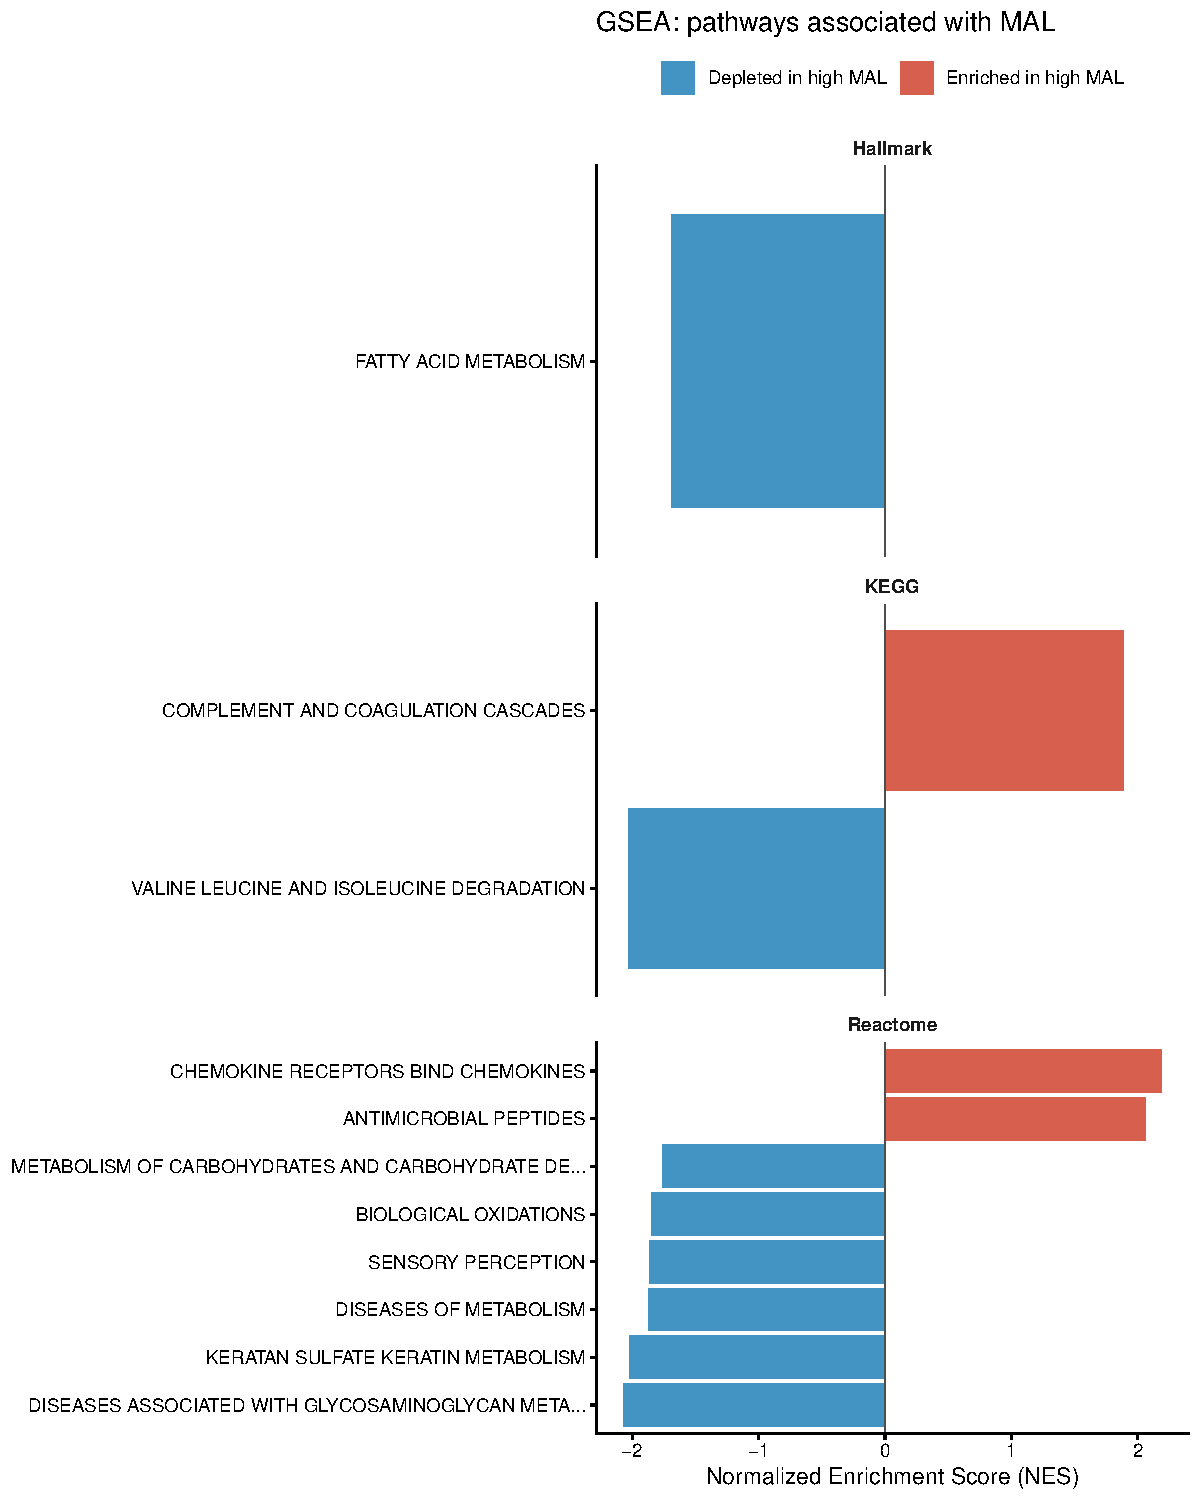
\includegraphics[width=0.75\textwidth]{Figure2B_GSEA.pdf}
  \caption{Gene Set Enrichment Analysis (GSEA) of MAL-associated plasma
    proteins across Hallmark, KEGG Legacy, and Reactome collections.
    Proteins ranked by MAL $t$-statistic ($n = 4{,}979$); bar length
    represents the Normalized Enrichment Score (NES). NES $> 0$ =
    enriched in high-MAL subjects; NES $< 0$ = depleted. Colour
    indicates direction. Only pathways with Benjamini--Hochberg adjusted
    $p < 0.05$ are shown ($n = 11$; 8 depleted, 3 enriched).}
\end{figure}

\subsection*{C. STRING Network}

Protein--protein interaction network for the 14 MAL-associated proteins.
Each node is one protein; node colour indicates direction of association
with MAL (red = enriched, blue = depleted) and node size encodes
$-\log_{10}(\text{FDR})$. An edge between two proteins indicates a known
or predicted functional interaction in STRING. Edge thickness scales with
the STRING combined confidence score. A cluster of connected nodes
indicates those proteins share a biological process; isolated nodes had
no qualifying interactions within this set.

\textbf{How calculated.}
14 FDR-significant proteins submitted to STRING~v11.5 human database
(human, species 9606). All interactions with combined confidence score
$\geq 200$ drawn to reveal subnetwork structure; edge thickness
proportional to score. Layout: Kamada--Kawai algorithm
(\texttt{igraph::layout\_with\_kk}).

\begin{figure}[H]
  \centering
  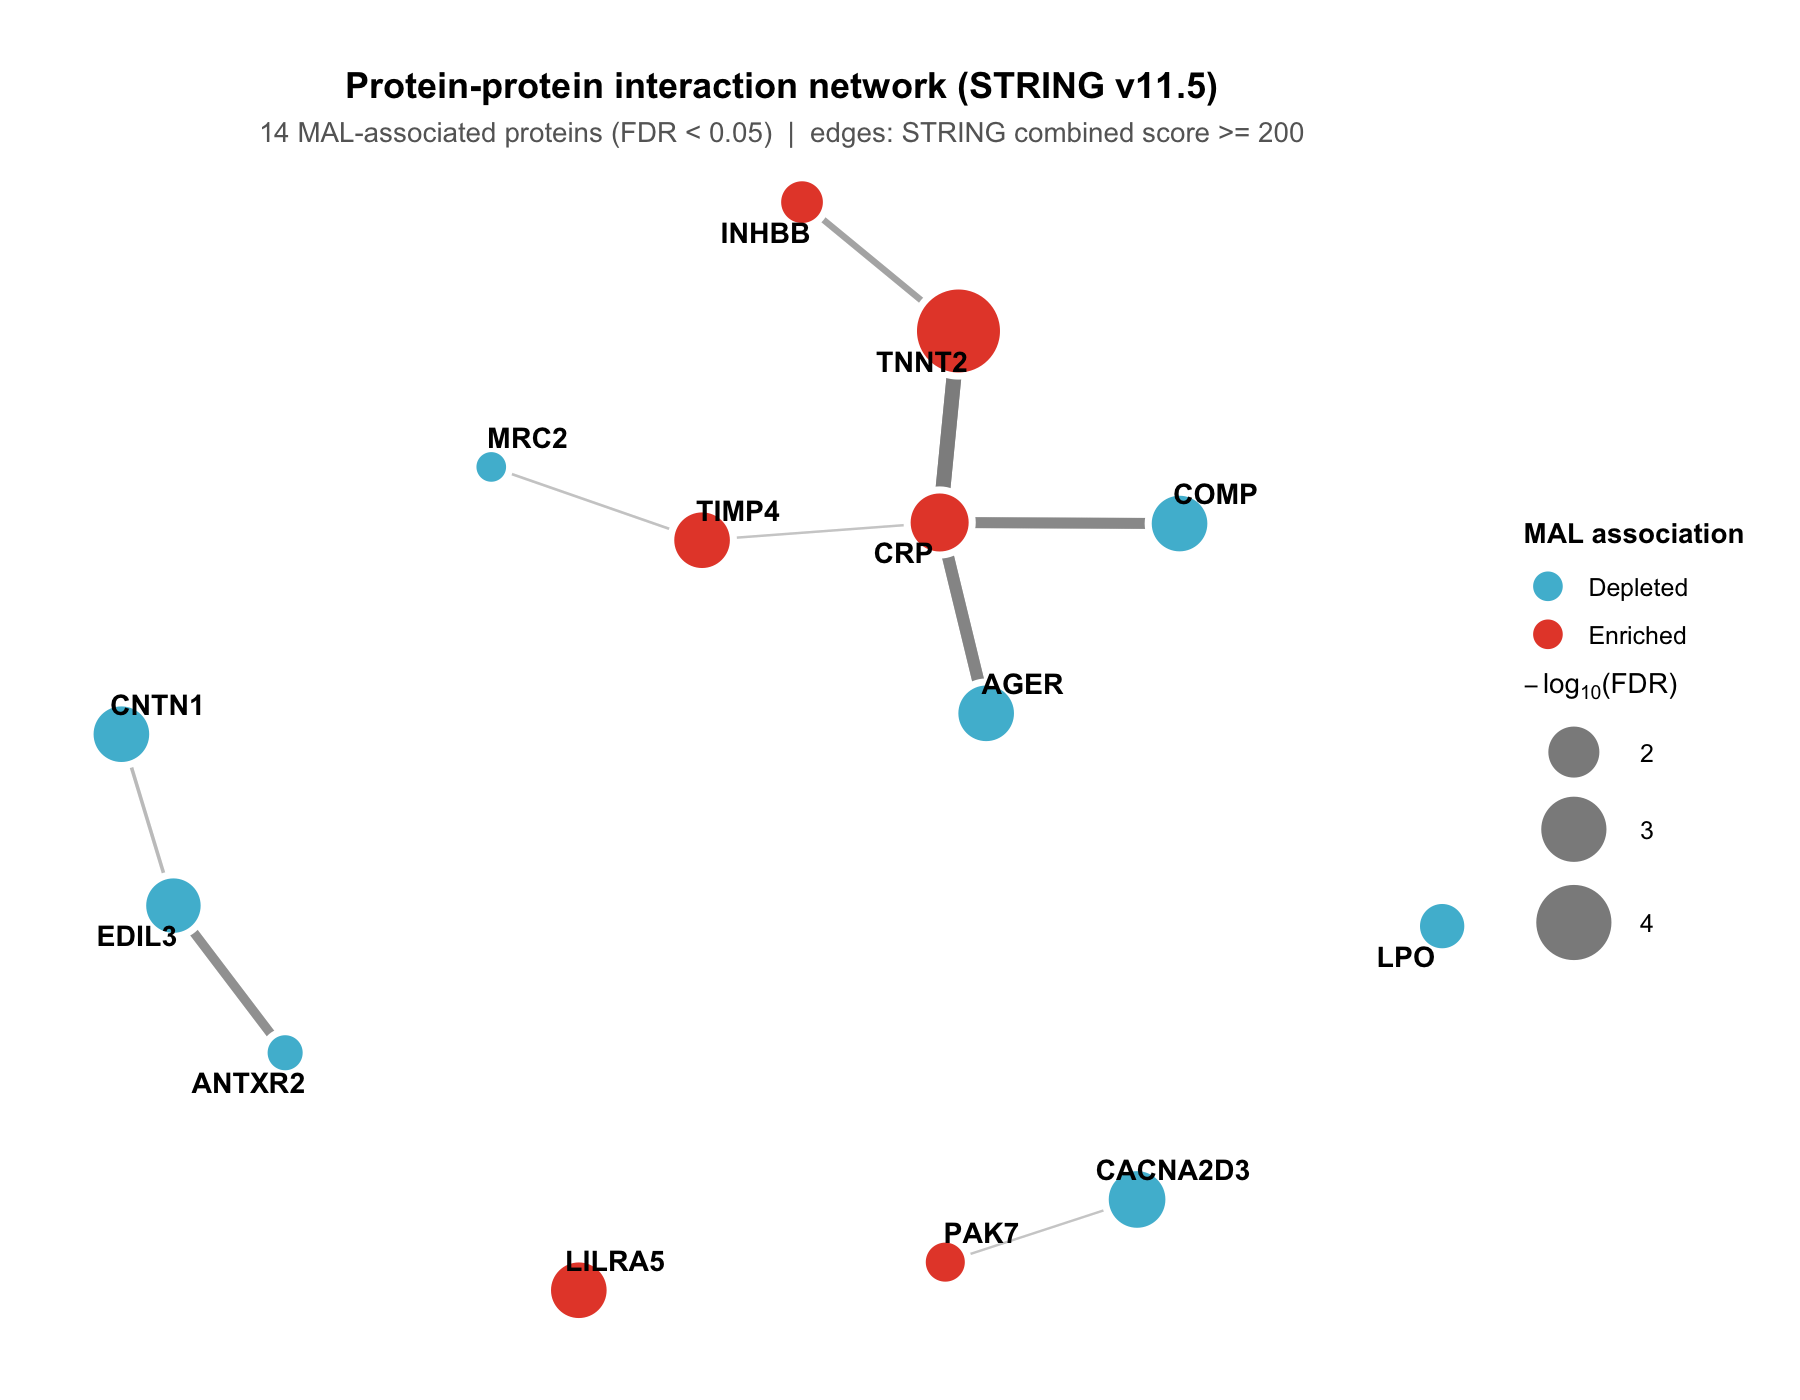
\includegraphics[width=0.85\textwidth]{Figure2C_STRING_network.png}
  \caption{Protein--protein interaction network for the 14 plasma
    proteins significantly associated with MAL (FDR $< 0.05$),
    constructed using STRING v11.5 (human, species 9606). Node colour:
    red = enriched with MAL, blue = depleted. Node size: $-\log_{10}(\text{FDR})$.
    Edges: STRING combined confidence score $\geq 200$; thickness
    proportional to score. Layout: Kamada--Kawai.}
\end{figure}

\subsection*{C2. MCL Clustering and Cluster Enrichment}

Markov Cluster Algorithm (MCL) clustering (inflation parameter = 2,
default) was applied to the STRING interaction network of the 14
MAL-associated proteins. MCL was run using the \texttt{MCL} R package
(\texttt{mcl()}, \texttt{addLoops=TRUE}, \texttt{inflation=2}) on the
binary adjacency matrix of the simplified subnetwork (combined score
$\geq 200$). Only clusters with $\geq 3$ proteins were retained;
pathway enrichment was retrieved from the STRING API across Gene
Ontology, KEGG, Reactome, and PubMed literature co-citation (text
mining); FDR computed by STRING using Benjamini--Hochberg against the
human proteome background. Full results
are in \texttt{STRING\_mcl\_clusters.csv} and
\texttt{STRING\_cluster\_enrichment.csv}.

Two clusters with $\geq 3$ proteins emerged. Cluster~1 ($n=3$: AGER,
COMP, CRP) co-enriches for published biomarker panels of carotid
stenosis and osteoarthritis (FDR $= 0.006$), reflecting shared
involvement in vascular and cartilage stress signalling. Cluster~2
($n=3$: ANTXR2, CNTN1, EDIL3) comprises extracellular matrix and cell
adhesion proteins; no significant pathway enrichment was returned by
STRING for this cluster. The remaining 8 proteins were unassigned.

\begin{table}[H]
\centering
\caption*{\textbf{MCL cluster enrichment summary.} Top enriched term
  per cluster (lowest FDR). Clusters with $\geq 3$ proteins shown.
  Full results in \texttt{STRING\_cluster\_enrichment.csv}.}
\begin{tabular}{clp{4.5cm}p{5.5cm}r}
\toprule
Cluster & $n$ & Members & Top term (source) & FDR \\
\midrule
1 & 3 & \small AGER, COMP, CRP
  & Biomarker panel for carotid stenosis / osteoarthritis
    (PubMed co-citation) & 0.006 \\
2 & 3 & \small ANTXR2, CNTN1, EDIL3
  & No significant enrichment & -- \\
\bottomrule
\end{tabular}
\end{table}

\begin{figure}[H]
\centering
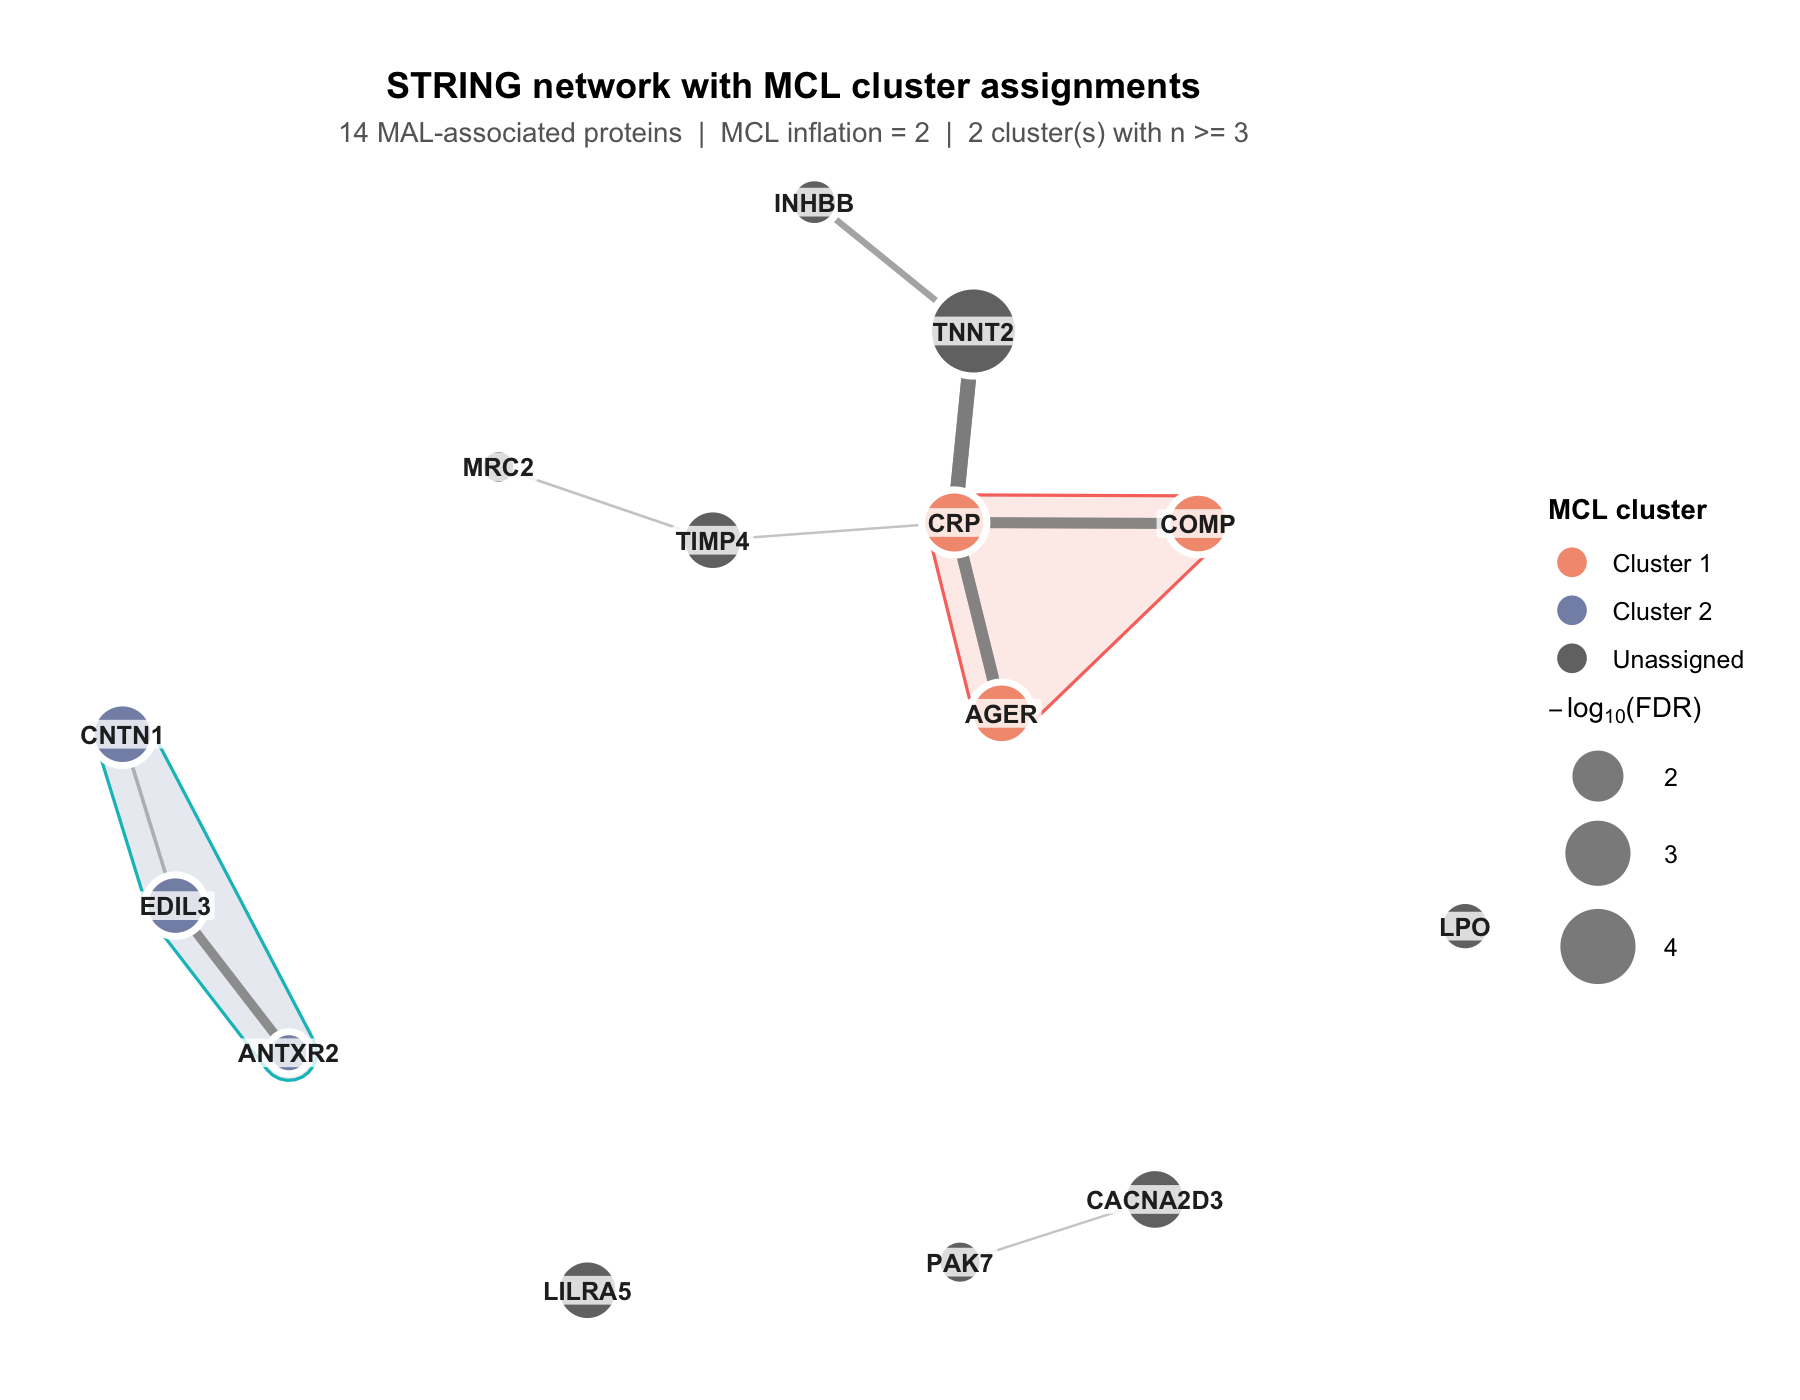
\includegraphics[width=0.90\textwidth]{Figure2C_STRING_MCL.png}
\caption*{\textbf{STRING network with MCL cluster assignments.}
  Nodes represent the 14 MAL-associated proteins (FDR $< 0.05$);
  edges: STRING combined score $\geq 200$; thickness proportional to
  score. Shaded hull indicates MCL cluster membership (inflation = 2).
  Cluster~1 (orange, $n=3$): AGER, COMP, CRP; co-cited as vascular/
  cartilage biomarkers in PubMed (FDR $= 0.006$).
  Cluster~2 (purple, $n=3$): ANTXR2, CNTN1, EDIL3; extracellular
  matrix and cell adhesion proteins; no significant pathway enrichment.
  Remaining 8 proteins unassigned (dark grey). Layout: Kamada--Kawai.}
\end{figure}

% =============================================================================
\section*{Proteomic Risk Score: Methods}

A single proteomic risk score is constructed for mechanical lung stress
and used for both the AIC model comparison and the causal
mediation analysis.

\textbf{MAL proteomic risk score (proRS).}
An adaptive LASSO ($\alpha = 1$) with MAL score (\texttt{meanmal}) as the
outcome was fitted on 70\% of the cohort
(\texttt{set.seed(42)}, $n_{\text{train}} = 914$,
$n_{\text{test}} = 392$). SomaScan RFU values were
log$_2$-transformed. Clinical covariates (age, sex, race, pack-years,
smoking status, CT scanner type, PC1--PC5, BMI) were included as
unpenalised fixed effects. Ridge regression on residualised \texttt{meanmal}
produced adaptive weights $w_j = 1/|\hat\beta^{\text{ridge}}_j|$;
10-fold inner cross-validation selected $\lambda_{\min}$; 572 proteins
were retained. Test $R^2 = 0.233$.

Post-selection OLS refitting yielded unbiased $\hat\beta_j$, SE, 95\% CI,
and $p$-values for each protein. The standardised score is:
\[
  \text{proRS}_i = \frac{\displaystyle\sum_{j} \hat\beta_j \cdot
    \log_2(\text{protein}_{ij}) \;-\; \bar{x}}
    {s}
\]
where $\bar{x}$ and $s$ are the mean and SD computed across all $n = 1{,}306$
subjects (\texttt{MAL\_PRS\_scaled}). The cross-validation curve
(Supplementary Figure~C) shows MSE as a function of $\log(\lambda)$,
and Supplementary Figure~D shows the concordance between
\texttt{MAL\_PRS\_scaled} and CT-derived \texttt{meanmal}
($R^2 = 0.543$, $n = 1{,}306$).

% =============================================================================
\section*{Association of Proteomic Risk Score with Emphysema Progression}

The MAL proRS (\texttt{MAL\_PRS\_scaled}; 572 proteins, test $R^2 = 0.233$
vs.\ \texttt{meanmal}) is evaluated on the held-out 30\% test set ($n = 392$)
to test whether the mechanistic protein signature of MAL independently
predicts future emphysema progression beyond clinical risk factors.
Three nested linear regression models use \texttt{pctprog} as the outcome;
scanner is included in M2 as a technical confounder.

\begin{align}
  \text{M1 (Clinical):} \quad
    &\texttt{pctprog} \;\sim\;
      \text{age} + \text{sex} + \text{race} + \text{smoking} +
      \text{pack-years} + \text{BMI} + \text{scanner} \notag \\[4pt]
  \text{M2 (proRS + scanner):} \quad
    &\texttt{pctprog} \;\sim\;
      \text{proRS} + \text{scanner} \notag \\[4pt]
  \text{M3 (Clinical + proRS):} \quad
    &\texttt{pctprog} \;\sim\;
      \text{proRS} + \text{age} + \text{sex} + \text{race} +
      \text{smoking} + \text{pack-years} + \text{BMI} + \text{scanner}
      \notag
\end{align}

\begin{table}[H]
\centering
\caption*{\textbf{Model comparison for predicting emphysema progression
  (\texttt{pctprog}) by AIC (test set, $n = 392$; lower = better fit).}
  Proteomic Risk Score = adaptive LASSO targeting \texttt{meanmal}
  (\texttt{MAL\_PRS\_scaled}, $\alpha = 1$, 572 proteins,
  10-fold inner CV; trained on 70\%, evaluated on 30\%).
  $\Delta$AIC relative to M1 (clinical reference);
  $\Delta \leq -2$ indicates meaningful improvement.}
\begin{tabular}{lrr}
\toprule
Model & AIC & $\Delta$AIC \\
\midrule
M1: Clinical (age, sex, race, smoking, pack-years, BMI, scanner) & $2{,}259.2$ & Reference \\
M2: proRS + scanner                                               & $2{,}286.6$ & $+27.4$ \\
M3: Clinical + proRS                                              & $2{,}245.7$ & $-13.5$ \\
\bottomrule
\end{tabular}
\end{table}

\noindent Effect sizes for \texttt{MAL\_PRS\_scaled}:
\begin{itemize}
  \item M2: $\hat\beta = 1.09\%$, 95\% CI $[0.67,\ 1.51]$, $p < 0.001$
  \item M3: $\hat\beta = 0.81\%$, 95\% CI $[0.40,\ 1.21]$, $p < 0.001$
\end{itemize}

\textbf{Key result.} The MAL proteomic risk score adds independent predictive
value for emphysema progression beyond clinical risk factors (M3: $\hat\beta
= 0.81\%$/SD, $p < 0.001$; $\Delta$AIC $= -13.5$, exceeding the $\leq -2$
threshold). These proteins were selected to predict CT-derived mechanical
lung stress, not emphysema progression, yet the score independently predicts
future CT density loss beyond smoking history, age, BMI, and spirometry.
This indicates that the blood protein signature of mechanical lung stress
carries prognostic information not captured by standard clinical covariates.

% =============================================================================
\section*{Figure 3: Proteomic Signature of Mechanical Stress Predicts Emphysema Progression}

Figure~3 shows a dose--response analysis of the MAL proteomic risk
score against emphysema progression. Subjects were divided into 10
equal deciles of \texttt{MAL\_PRS\_scaled} ($\approx 131$ subjects per
decile; D1 = lowest score, D10 = highest). The x-axis shows the mean
proteomic risk score within each decile bin (SD units); the y-axis
shows the mean \texttt{pctprog} (percentage of lung voxels showing
emphysema progression) for that bin. A linear regression line with
95\% confidence band is overlaid. Error bars on each point are
95\% CI (mean $\pm 1.96 \times$ SE). No covariates were adjusted.

\textbf{How calculated.}
\texttt{MAL\_PRS\_scaled} is the standardised adaptive LASSO score
described in the Proteomic Risk Score Methods section (572 proteins,
outcome = \texttt{meanmal}, trained on 70\% of the cohort). All
$n = 1{,}306$ subjects are ranked by their score and divided into 10
equal-sized groups (deciles; $\approx 131$ subjects each). Within each
decile, the mean score (\textit{x}) and mean \texttt{pctprog} (\textit{y})
are computed. Error bars are 95\% CI ($\text{mean} \pm 1.96 \times$
SE, where SE $= \text{SD}/\sqrt{n}$). The overlaid line is a simple
linear regression of \texttt{pctprog} on \texttt{MAL\_PRS\_scaled}
across all $n = 1{,}306$ subjects; the shaded band is the 95\%
confidence region. No covariates are adjusted in this descriptive
plot. The D10/D1 ratio compares the mean \texttt{pctprog} in the
highest vs.\ lowest decile; the trend $p$-value is from the regression
slope.

\textbf{Key result.}
The proteomic risk score shows a near-monotone dose--response with
emphysema progression: subjects in the highest decile of the blood
score had $3.1\times$ more lung progression than those in the lowest
(D10/D1 $= 3.1\times$, $p = 1.52 \times 10^{-40}$). This dose--response
arises from a score derived entirely from plasma proteins targeting
CT-measured mechanical stress, demonstrating that the blood signature
of MAL independently stratifies patients by future emphysema
progression.

\begin{figure}[H]
  \centering
  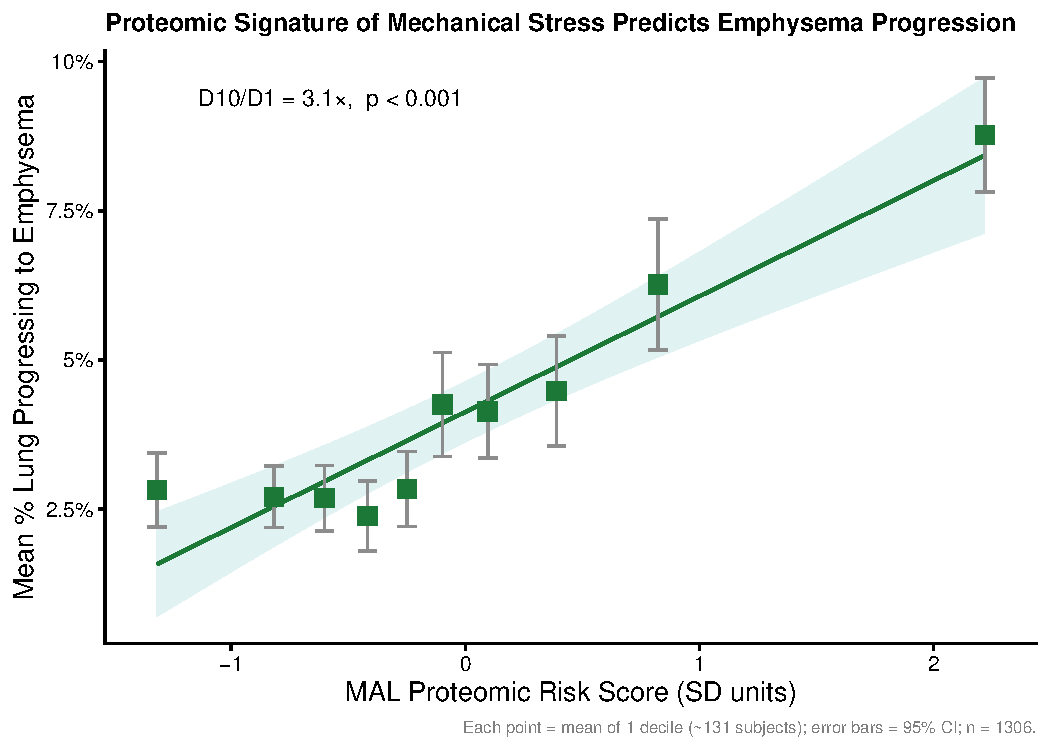
\includegraphics[width=0.72\textwidth]{Figure3_quartile_plot.pdf}
  \caption{Mean \% of lung progressing to emphysema (\texttt{pctprog},
    y-axis) across 10 equal deciles of the MAL proteomic risk score
    (\texttt{MAL\_PRS\_scaled}, x-axis, SD units; $n = 1{,}306$).
    Each green square is the mean of one decile ($\approx 131$
    subjects); error bars: 95\% CI of the decile mean. Line: linear
    regression of \texttt{pctprog} on \texttt{MAL\_PRS\_scaled} across
    all subjects; shaded band: 95\% confidence region for the
    regression line (i.e., uncertainty in the fitted mean at each score
    value, not a prediction interval for individual subjects).
    D10/D1 $= 3.1\times$, $p = 1.52 \times 10^{-40}$.}
\end{figure}

% =============================================================================
\section*{Table 2: Causal Mediation}

The analysis decomposes the total effect of MAL on emphysema progression
into a direct path (NDE) and a path through the blood protein score
(NIE). NDE = how much of the MAL effect goes through pathways other than
the protein score. NIE = how much goes through the protein score.
All effects are in HU (Hounsfield Units), the CT density scale. More
negative HU = lower lung density = more emphysema. A difference of 1 HU
is a small change; the SD of progression in this cohort is $\sim$7 HU.

\begin{itemize}
  \item \textbf{NDE = $-$0.55 HU, $p = 0.941$:} MAL's direct effect
    on progression is non-significant once blood protein changes are
    accounted for. The 95\% CI spans zero $[-14.96,\ 13.86]$,
    consistent with no independent direct effect.
  \item \textbf{NIE = 13.93 HU, $p = 0.002$:} the protein risk score
    mediates a large and significant portion of the MAL effect. A
    one-unit increase in MAL is associated with 13.93 HU more
    progression through the protein pathway.
  \item \textbf{Proportion mediated $\approx 100\%$:} the indirect
    path through blood proteins explains essentially all of the
    MAL--progression relationship. The NDE is non-significant,
    consistent with complete mediation.
  \item \textbf{Total effect = 13.38 HU:} NDE + NIE; the protein
    pathway accounts for the entire effect.
\end{itemize}

\textbf{How calculated.}
Pathway tested: MAL $\to$ Proteomic Risk Score $\to$ Emphysema
Progression. Fitted using the \texttt{medflex} R package (natural
effects framework) with robust sandwich standard errors.

Two models fitted internally by \texttt{medflex}:
\[
  \text{Imputation model: }
  \Delta\rho \;\sim\; \texttt{meanmal} \times \text{proRS} + \text{covariates}
\]
\[
  \text{Natural effects model: }
  \Delta\rho \;\sim\; \texttt{meanmal}_0 + \texttt{meanmal}_1 + \text{covariates}
\]
$\texttt{meanmal}_0$ is the MAL value at which the mediator (proRS) is
set (direct path); $\texttt{meanmal}_1$ is the actual MAL value driving
the outcome (indirect path). The difference between them isolates the
mediated portion.

\begin{table}[H]
\centering
\caption*{\textbf{Table 2.} Causal mediation of the MAL--emphysema
  progression relationship through the Proteomic Risk Score (proRS),
  estimated using the natural effects framework (\texttt{medflex} R
  package, robust sandwich SE, $n = 1{,}306$). NDE (Natural Direct
  Effect) = portion of MAL's effect on $\Delta$CT lung density not
  operating through the proRS. NIE (Natural Indirect Effect) = portion
  operating through the proRS. Proportion mediated = NIE / total effect.
  All effects in HU (Hounsfield Units; negative = more emphysema).}
\begin{tabular}{lrrrr}
\toprule
Effect & Estimate (HU) & 95\% CI & $z$ & $p$ \\
\midrule
Natural Direct Effect (NDE)   & $-0.55$  & $[-14.96,\ 13.86]$ & $-0.07$ & $0.941$ \\
Natural Indirect Effect (NIE) & $+13.93$ & $[5.26,\ 22.60]$   & $+3.15$ & $0.002$ \\
Total effect                  & $+13.38$ & \multicolumn{3}{c}{---} \\
Proportion mediated           & \multicolumn{4}{c}{${\approx}100\%$} \\
\bottomrule
\end{tabular}
\end{table}

\textbf{Key result.} The proteomic risk score fully mediates the
effect of MAL on emphysema progression (NIE = 13.93 HU,
$p = 0.002$). The direct path is non-significant once the protein
pathway is accounted for (NDE = $-$0.55 HU, $p = 0.941$), consistent
with complete mediation.

% =============================================================================
\section*{Supplement}

\subsection*{Supplementary Tables}

\begin{itemize}
  \item \textbf{S1: All differential expression results} (4,979
    proteins): gene, target, $\hat\beta$, SE, $t$, $p$, FDR. \\
    File: \texttt{MAL\_omics/mal\_de\_results.csv}

  \item \textbf{S2: proRS weights} (MAL-targeting LASSO proteins): gene, target,
    $\hat\beta_{\text{OLS}}$, 95\% CI, $p$. \\
    File: \texttt{MAL\_omics/mal\_risk\_score\_weights.csv}

  \item \textbf{S3: Per-protein mediation} (MAL-targeting LASSO proteins): NDE, NIE,
    total, proportion mediated, NIE $p$. \\
    File: \texttt{MAL\_omics/mal\_mediation\_supp.csv}

    Of 199 converged proteins (from the 572 proRS proteins), 10 reached
    NIE $p < 0.05$. Proportions mediated range from $-9\%$ to $18\%$;
    EPHB2 shows negative mediation (suppression).

\begin{table}[H]
\centering
\caption*{\textbf{Supplementary Table S3.} Per-protein causal mediation:
  MAL $\to$ individual protein $\to$ emphysema progression. Only proteins
  with NIE $p < 0.05$ shown ($n = 10$ of 202 converged). NDE = Natural
  Direct Effect; NIE = Natural Indirect Effect. All effects in HU.
  Proportion mediated = NIE / (NDE + NIE). \texttt{medflex}, robust SE,
  $n = 1{,}306$.}
\begin{tabular}{llrrrrrr}
\toprule
Gene & Target & NDE (HU) & NDE $p$ & NIE (HU) & NIE $p$ & \% Mediated \\
\midrule
TREM2    & TREM2            & $+13.67$ & $0.011$ & $+2.78$ & $0.012$ & $17\%$ \\
MANSC4   & MANS4            & $+14.23$ & $0.008$ & $+1.73$ & $0.012$ & $11\%$ \\
EPHB2    & EPHB2            & $+20.54$ & $<0.001$ & $-1.64$ & $0.016$ & $-9\%$ \\
DEFA5    & HD-5             & $+14.61$ & $0.006$ & $+1.66$ & $0.017$ & $10\%$ \\
ADH7     & ADH7             & $+15.01$ & $0.006$ & $+1.79$ & $0.021$ & $11\%$ \\
ADAMTS5  & ADAMTS-5         & $+15.37$ & $0.004$ & $+1.22$ & $0.021$ & $7\%$  \\
INHBB    & Inhibin $\beta$B & $+13.07$ & $0.020$ & $+2.88$ & $0.022$ & $18\%$ \\
SCG3     & SCG3             & $+13.46$ & $0.015$ & $+2.65$ & $0.029$ & $16\%$ \\
MSMP     & PSMP             & $+13.80$ & $0.011$ & $+1.78$ & $0.034$ & $11\%$ \\
PDCD1    & PD-1             & $+16.26$ & $0.002$ & $+0.76$ & $0.048$ & $4\%$  \\
\bottomrule
\end{tabular}
\end{table}
\end{itemize}

\subsection*{Supplementary Figures}

\begin{itemize}
  \item \textbf{Supp Figure A: Forest plot, proteins $\sim$ MAL.}
    Top 30 proteins by $|t\text{-statistic}|$, showing $\hat\beta$
    (log$_2$ RFU per unit MAL) with 95\% CI. Red = positively associated;
    blue = negatively associated with MAL.

\begin{figure}[H]
  \centering
  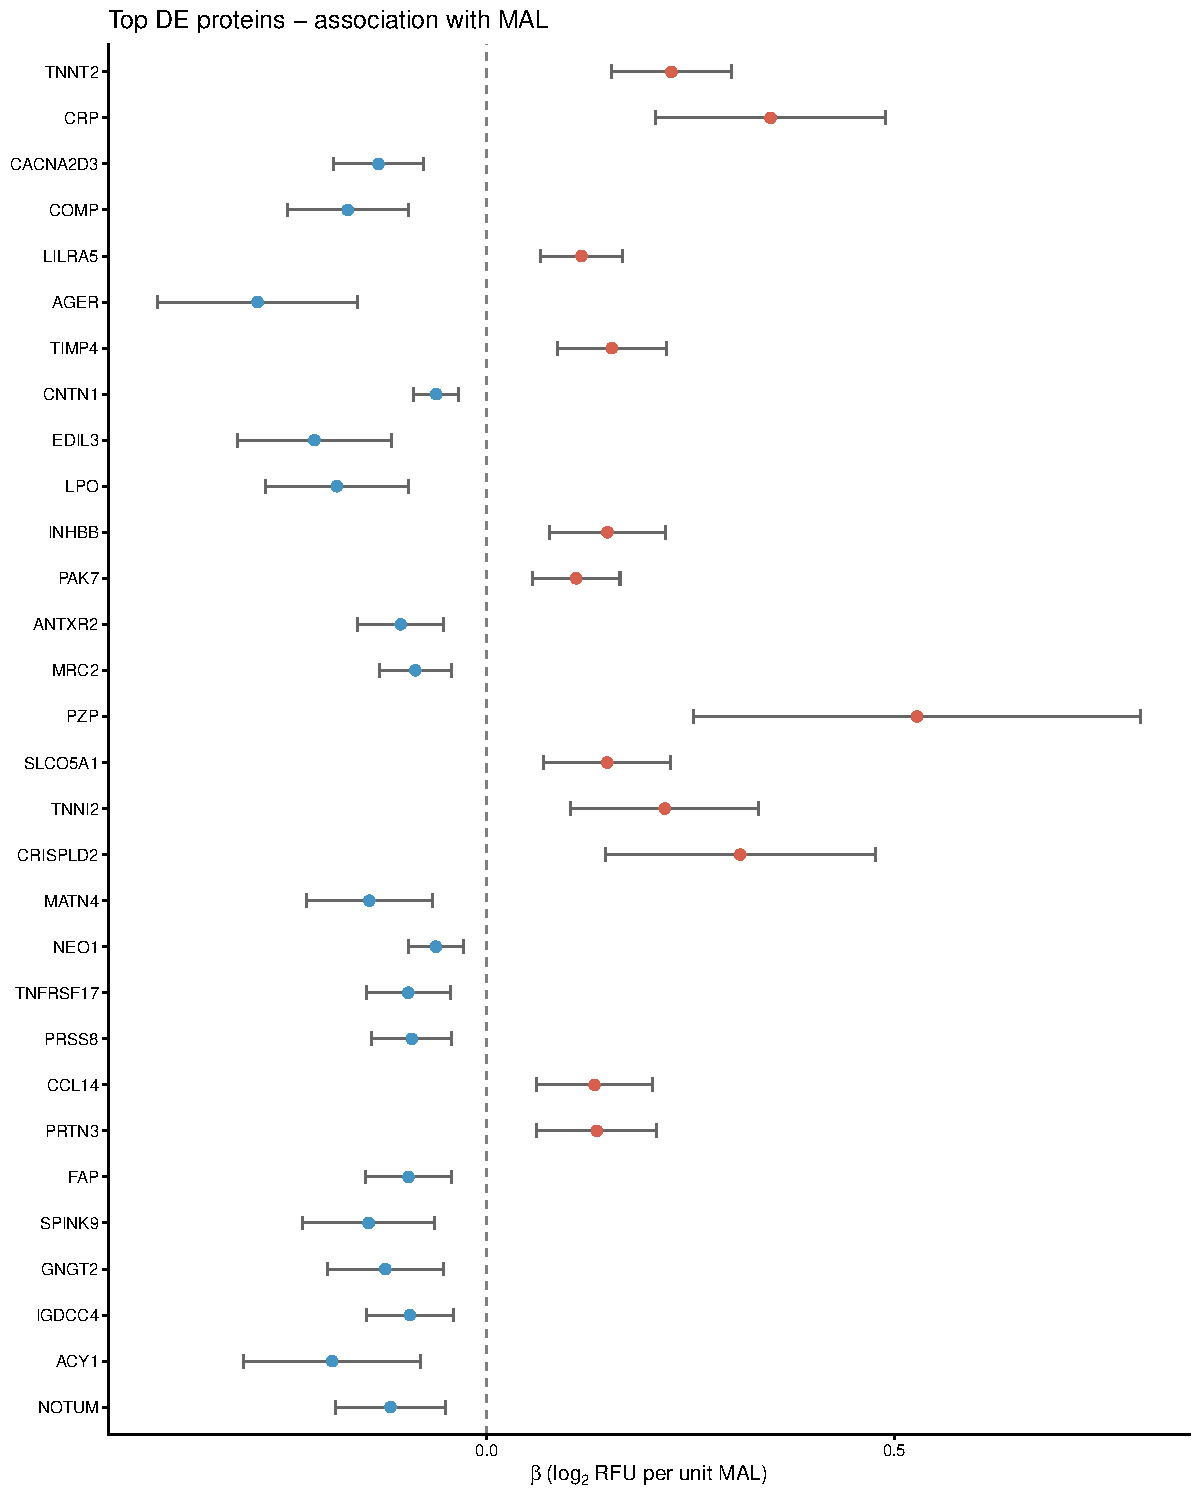
\includegraphics[width=0.75\textwidth]{SuppFig_forest_MAL.pdf}
  \caption*{\textbf{Supplementary Figure A.} Forest plot of the top 30
    proteins most significantly associated with MAL score (ranked by
    $|t\text{-statistic}|$). Points show $\hat\beta$ (log$_2$ RFU per
    unit MAL) with 95\% CI, from the model: $\log_2(\text{protein}) \sim
    \texttt{meanmal} + \text{age} + \text{sex} + \text{race} +
    \text{pack-years} + \text{smoking} + \text{BMI} + \text{scanner} +
    \text{PC1--PC5}$. Red = positively associated; blue = negatively
    associated with MAL. Vertical dashed line at zero.}
\end{figure}

  \item \textbf{Supp Figure B: Forest plot, proteins $\sim$ emphysema progression.}
    Same 30 proteins, association with emphysema progression
    (\texttt{Change\_lung\_density\_vnb\_P2\_P3}) adjusted for baseline
    lung density and covariates.

\begin{figure}[H]
  \centering
  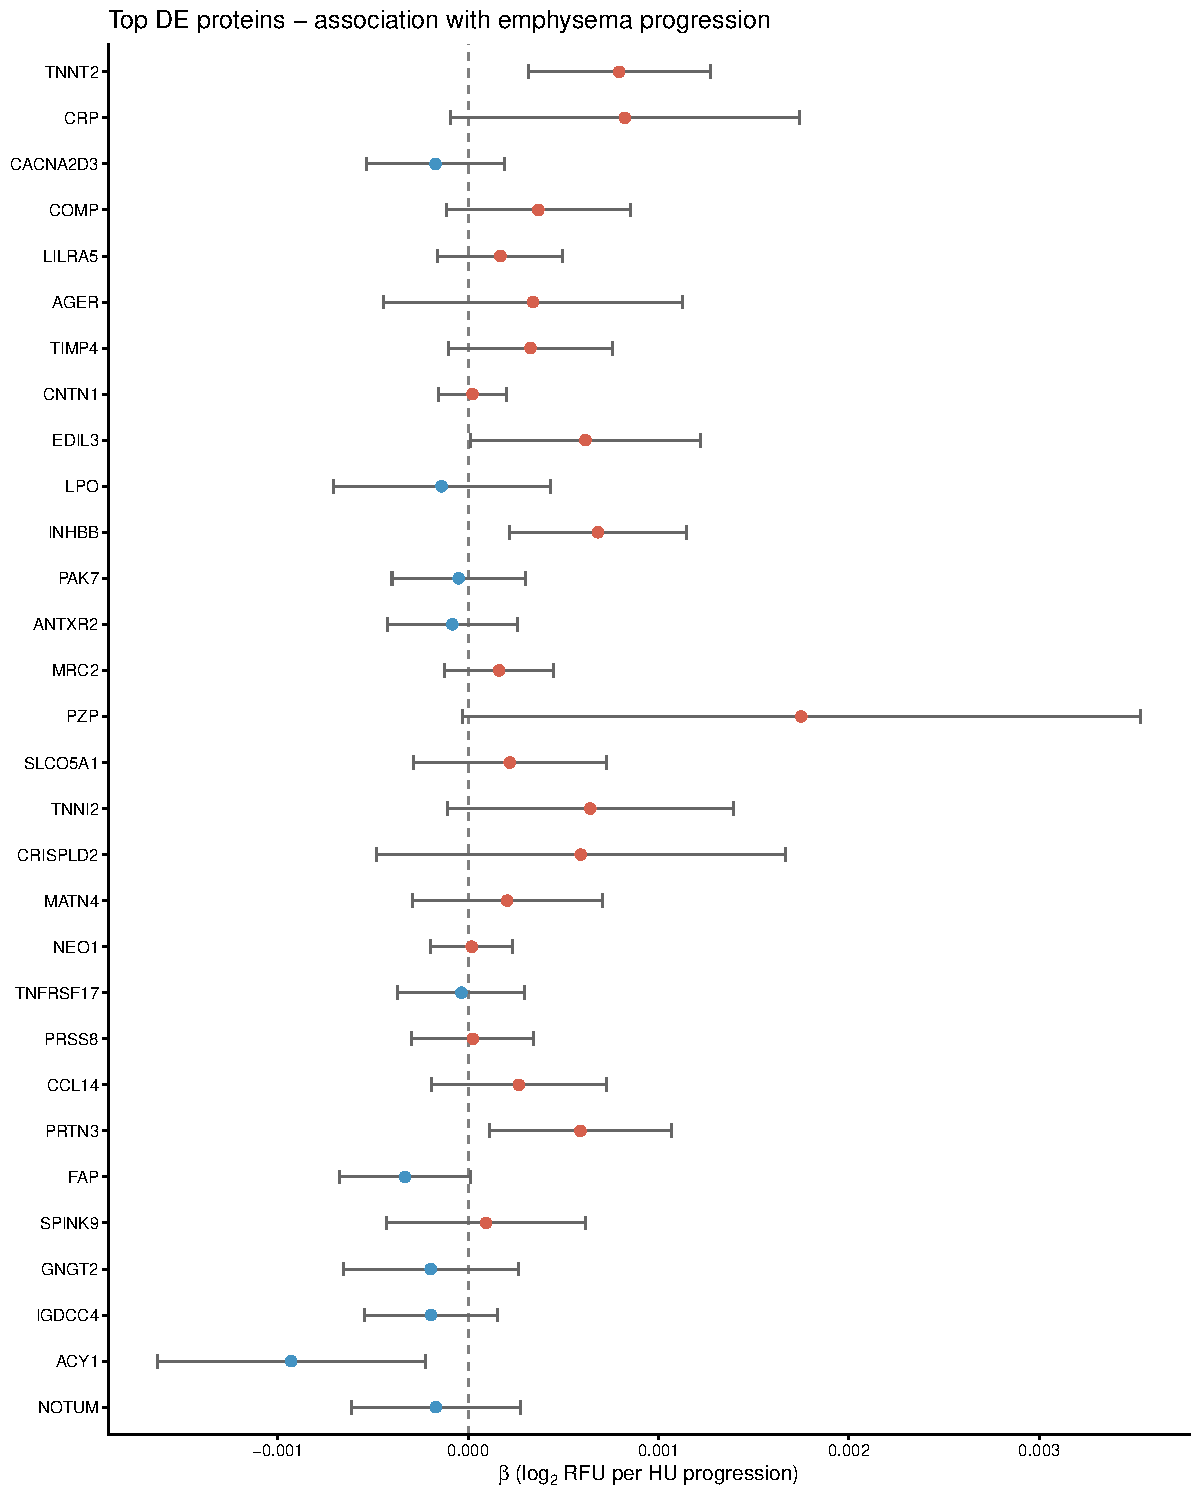
\includegraphics[width=0.75\textwidth]{SuppFig_forest_progression.pdf}
  \caption*{\textbf{Supplementary Figure B.} Forest plot of the same top
    30 MAL-associated proteins showing their association with emphysema
    progression. Points show $\hat\beta$ (log$_2$ RFU per HU progression)
    with 95\% CI, from the model: $\log_2(\text{protein}) \sim
    \texttt{Change\_lung\_density\_vnb\_P2\_P3} +
    \texttt{lung\_density\_vnb\_P2} + \text{age} + \text{sex} +
    \text{race} + \text{pack-years} + \text{smoking} + \text{BMI} +
    \text{scanner} + \text{PC1--PC5}$. Vertical dashed line at zero.}
\end{figure}

  \item \textbf{Supp Figure C: Adaptive LASSO cross-validation curve.}
    Mean squared error from 10-fold CV plotted against $\log(\lambda)$
    for the MAL-targeting adaptive LASSO. Shaded band: $\pm 1$ SE.
    Dashed red line: selected $\lambda_{\min}$ and the number of
    proteins retained at that penalty.

\begin{figure}[H]
  \centering
  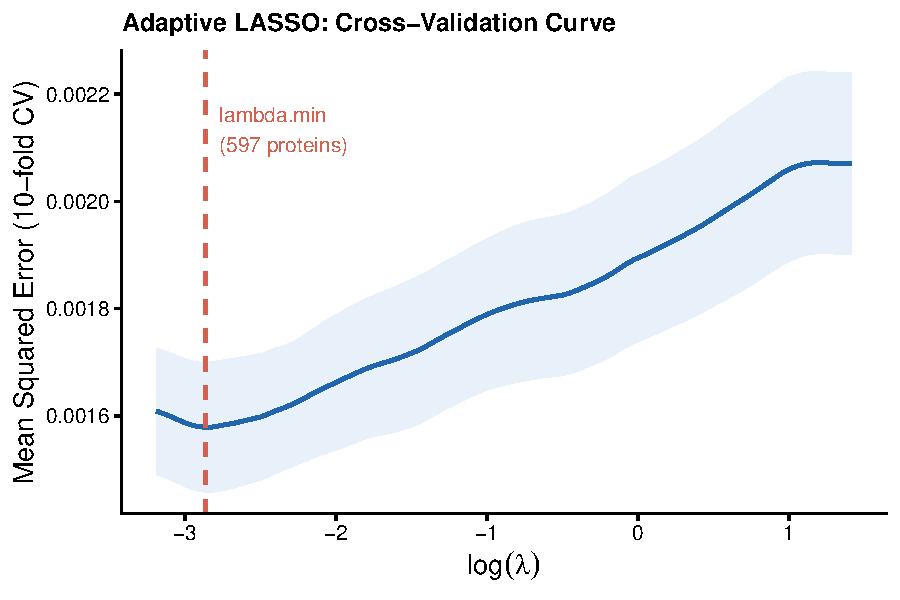
\includegraphics[width=0.60\textwidth]{SuppFig_CV_curve.pdf}
  \caption*{\textbf{Supplementary Figure C.} Cross-validation curve
    for the adaptive LASSO (proRS\textsubscript{MAL}). MSE (10-fold CV)
    is plotted against $\log(\lambda)$; shaded band shows $\pm 1$ SE.
    The dashed line marks $\lambda_{\min}$, the penalty that minimises
    CV-MSE and determines how many proteins are retained in the risk
    score.}
\end{figure}

  \item \textbf{Supp Figure D: Proteomic risk score vs.\ CT MAL score.}
    Scatter of the MAL-targeting proteomic risk score (SD units, x-axis)
    against CT-derived \texttt{meanmal} (y-axis) for all $n = 1{,}306$
    subjects. Fitted regression line with 95\% CI band shown.
    $R^2 = 0.543$ confirms that the blood protein signature captures
    a meaningful fraction of CT-measured MAL variance.

\begin{figure}[H]
  \centering
  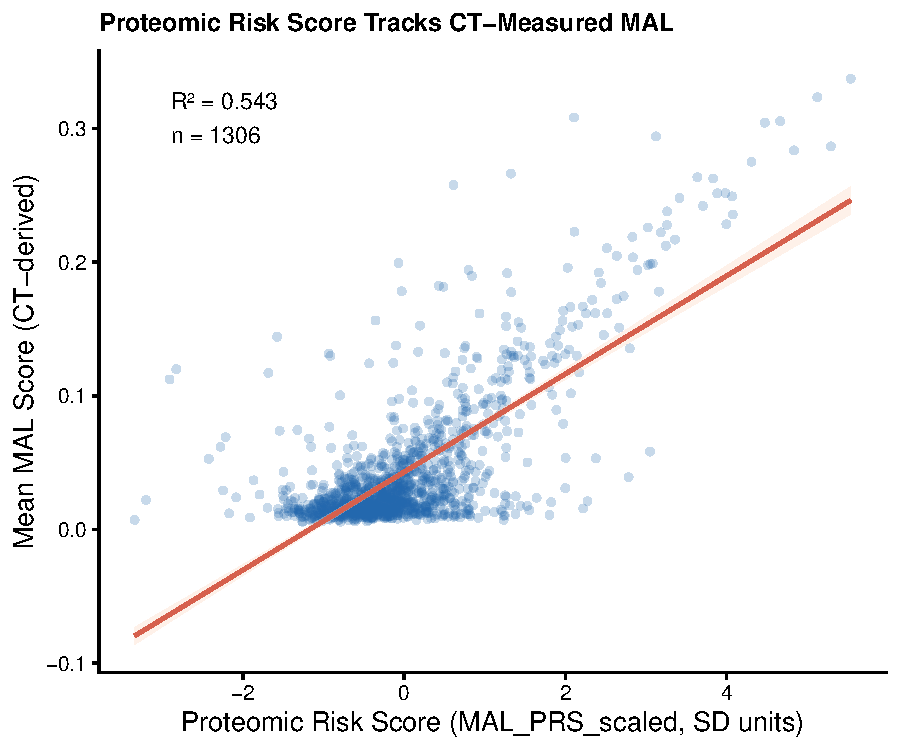
\includegraphics[width=0.60\textwidth]{SuppFig_PRS_vs_MAL.pdf}
  \caption*{\textbf{Supplementary Figure D.} Concordance between the
    MAL-targeting proteomic risk score (\texttt{MAL\_PRS\_scaled},
    derived from 572 blood proteins) and the CT-derived MAL score
    (\texttt{meanmal}). Each point is one subject ($n = 1{,}306$);
    regression line with 95\% CI shown. $R^2 = 0.543$.}
\end{figure}

\end{itemize}

\end{document}
